\documentclass[12pt]{article}
\usepackage{amsmath,amsthm}
\usepackage{mathtools}
\usepackage{tikz}

\DeclareGraphicsExtensions{.png}

\newtheorem{thm}{Theorem}
\newtheorem{lem}[thm]{Lemma}

\begin{document}

\begin{center}
\large\bf University of Waterloo\\
CS~798 --- Mathematical Foundations of Computer Networking\\
Winter 2014\\
Assignment 1\\
Siwei Yang - 20258568\\
\end{center}
\bigskip

\begin{enumerate}
\item{Problem 1}

\begin{enumerate}
\item{} The activities in a system are observed for a time period of length L (from 0 to L).
Let:
\begin{itemize}
\item n = number of jobs arrived in (0, L) = number of jobs processed in (0, L) 
\item $a_j$ = probability that an arriving job sees j jobs in the system
\item $d_j$ = probability that a departing job leaves behind j jobs in the system
\end{itemize}
There are no group arrivals (i.e., jobs arrive one after another). Show that $a_j$ = $d_j$ for all j.

Let $h_i$ be the number of jobs in the system when the $i^{th}$ job arrives, and $b_i$ be the number of jobs in the system when the $i^{th}$ job leaves the system. Of course, realistically, the order job arrives and departures have nothing to do with each other. However

\begin{lem}
we can alter the order job leaves the system without affecting $a_j, d_j$
for any scenario
\end{lem}

So, re-order the job departures so that it is always the last arriving job that leaves the system first. This gurantees every job sees the same number of jobs when both arriving and leaving the system. In other words, for any job, jobs arriving after it will leave system before it too. And jobs it sees on arrival will not leave system until it leaves. Therefore we have

\begin{equation}
\forall i . h_i = b_i
\end{equation}

Also we know that

\begin{equation}
a_i = \mid \{h_j \mid h_j = i\} \mid
\end{equation}

\begin{equation}
d_i = \mid \{b_j \mid b_j = i\} \mid
\end{equation}

Thus, given $h_i = b_i$, we can conclude that $a_i = d_i$ for all $i$.
\item{} Suppose arrivals occur in groups of two (i.e., we always see two jobs arriving at the same time), and we assume that both arriving jobs see the same number of jobs in the system. Is the relationship $a_j$ = $d_j$ for all j still true for this case? Explain your answer.

The relationship is not true any more. A simple counter example can be given for the case that only 2 jobs in total. So we have:
\begin{equation}
h_0=h_1=0 \text{ and }b_0=1,b_1=0
\end{equation}
Therefore, we calculate $a_0=1$ and $d_0=\frac{1}{2}, d_1=\frac{1}{2}$ which are not equal.

\end{enumerate}

\medskip

\item{Problem 2}

Suppose there are n arrivals in a time period of length L (from 0 to L), and the $n^{th}$ arrival (or last arrival) occurs at time L. Let $t_1$ be the time between 0 and the time of the first arrival, and $t_i$ be the interarrival time between the $(i-1)^{st}$ and $i^{th}$ arrivals, $i = 2, 3, \dotsc, n$
\begin{enumerate}
\item{} Let X be the time until the next arrival. Plot X as a function of time t for $0 \le t \le L$.

\item{} Let $E[Y] = \frac{1}{n} * \sum^{n}_{i=1}{t_i}$ and $E[Y^2] = \frac{1}{n} * \sum^{n}_{i=1}{t_i^2}$ be the mean and second moment of the interarrival time, respectively. Using the plot in part (a), obtain an expression for E[X], the mean of X, as a function of E[Y] and E[Y2].
\begin{equation}
E[X] * L = \int_{0}^{L}{X}
\end{equation}

In other words, $E[X] * L$ equals to the bounded regions in plot of part a.
\begin{equation}\label{eq:region}
E[X] * L = \sum_{1}^{n}{\frac{t^2}{2}}
\end{equation}

and we know that
\begin{equation}\label{eq:region-sum}
E[Y] * n = L, E[Y^2] * n = \sum^{n}_{i=1}{t_i^2}
\end{equation}

Combine \ref{eq:region} and \ref{eq:region-sum} together, we end up with
\begin{equation}
E[X] = \frac{E[Y^2]}{2 * E[Y]}
\end{equation}

\end{enumerate}

\item{Problem 3}
\begin{enumerate}
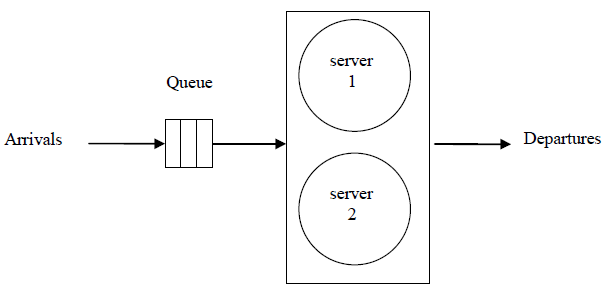
\includegraphics[scale=0.9]{a1q3.png}
\item{} Consider a single server queue model with two classes of jobs. Let $n_j$ = number of class j jobs arrived in $(0, L)$ = number of class j jobs processed in $(0, L)$, j = 1, 2. Also let $x_{ij}$ be the service time of the $i^{th}$ class j job. Obtain analytic results for $U_j^{'}$, the utilization of the server by class j jobs, j = 1, 2.

\item{} Consider a queueing model with a single queue and two parallel servers (see Figure below). Let n = number of jobs arrived in (0, L) = number of jobs processed in (0, L). Also let $x_i$ be the service time of the $i^{th}$ job. Is it possible to obtain analytic results for $U_i$, the utilization of server i, i = 1, 2? Explain your answer.

\end{enumerate}


\end{enumerate}

\end{document}

